\chapter{集合及其运算}


  \begin{Def}
    通常把一些互不相同的东西放在一起所形成的整体叫做一个集合。构成集合的每个东西叫做集合的元素。
给定一个集合$A$和一个元素$a$,用$a \in A$表示$a$是$A$的一个元素,用$a \notin A$表示$a$不是$A$的一个元素。
  \end{Def}

  有两种方法表示一个集合:
\begin{enumerate}
\item 把构成集合的那些元素全部列出来
  \begin{itemize}
  \item $A = \{1, 2, 3\}$
\item $C = \{a, b, c, \ldots, z\}$
  \end{itemize}
\item 用概括集合中各元素的属性来表示集合$\{x|P(x)\}$
\begin{itemize}
\item $E = \{n|n \in \mathcal{Z} \land n\text{ is even}\}$,这里$\land$表示“并且”,$E$还可以等价的表示为$E = \{n \in \mathcal{Z} | n\text{ is even}\}$
\end{itemize}
\end{enumerate}

存在一个集合,该集合中不包含任何元素,称为空集,记为$\phi$。
  \begin{Thm}
   空集为任一个集合的子集且空集是唯一的。 
  \end{Thm}

  
    \begin{Def}
    设$A$,$B$为两个集合,如果$A$中的每个元素都是$B$中的元素,则称$A$为$B$的
子集,记为$A \subseteq B$; 如果$A \subseteq B$且存在$x\in B$使得$x \notin A$,则称$A$为$B$的真子集,记为$A\subset B$。    
\end{Def}
\begin{itemize}
  \item   $\{1,2,4\} \subseteq \{1,2,3,4,5\}$
\item $\{1,2,4\} \subset \{1,2,3,4,5\}$
  \end{itemize}

    \begin{Def}
    设$A$,$B$为两个集合,如果$A \subseteq B$且$B \subseteq A$,则称$A$与$B$相等,并记为$A=B$。
  \end{Def}
    \begin{itemize}
  \item   $\{1,2,3,4,5\} = \{3,4,2,1,5\}$
\item $\{x \in \mathcal{R} | x^2 -5x + 6 = 0\} = \{2,3\}$
  \end{itemize}

\begin{Def}
  集合$S$的所有子集构成的集合称为$S$的幂集,记为$2^S$或者$\mathcal{P}(S)$。
\end{Def}
\begin{Example}
  设$S=\{1,2,3\}$,则$2^s=\{\phi, \{1\},\{2\},\{3\},\{1,2\},\{1,3\},\{2,3\},\{1,2,3\}\}$。
\end{Example}

{
\flushleft
\begin{minipage}{0.70\linewidth}
  \begin{Def}
    设$A,B$为任意的两个集合,至少属于集合 $A$ 与集合$B$之一的那些元素构成的集合称为$A$与$B$的并集,记为$A \cup B$。
  \begin{equation*}
      A\cup B = \{x|x \in A \lor x \in B\} 
    \end{equation*}
    (这里$\lor$表示“或者”)
  \end{Def}
\end{minipage}
\begin{minipage}{0.29\linewidth}
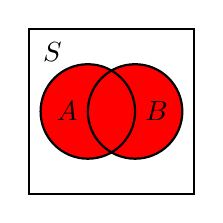
\begin{tikzpicture}[thick, scale=0.3]
  \draw (-3.5, -3.5) rectangle (3.5, 3.5);
  \filldraw[fill=red] (-1,0) circle [radius=2cm]
               (1,0) circle [radius=2cm];
  \draw (-1,0) node[left] {$A$};
  \draw (1,0) node[right] {$B$};
  \draw (-2.5,2.5) node {$S$};
\end{tikzpicture}
 \end{minipage}
}
\begin{Example}
  $\{1,2\} \cup \{2,3\} = \{1,2,3\}$
\end{Example}

{\flushleft
\begin{minipage}{0.70\linewidth}
  \begin{Def}
    设$A,B$为任意的两个集合,由既属于集合 $A$ 又属于集合$B$的所有元素构成的集合称为$A$与$B$的交集,记为$A \cap B$。
    \begin{equation*}
      A\cap B = \{x|x \in A \land x \in B\}
    \end{equation*}
  \end{Def}
\end{minipage}
\begin{minipage}{0.29\linewidth}
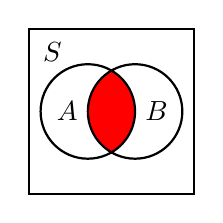
\begin{tikzpicture}[thick, scale=0.3]
  \draw (-3.5, -3.5) rectangle (3.5, 3.5);
  \fill[red] (-0.01, 0 |- -60:2cm) arc [start angle=-60, end angle = 60, radius = 2cm];
  \fill[red] (0.01, 0 |- 120:2cm) arc [start angle=120, end angle = 240, radius = 2cm];
  \draw (-1,0) circle [radius=2cm]
               (1,0) circle [radius=2cm];
  \draw (-1,0) node[left] {$A$};
  \draw (1,0) node[right] {$B$};
  \draw (-2.5,2.5) node {$S$};
\end{tikzpicture}
  \end{minipage}
    \begin{Example}
        $\{1,2\} \cap \{2,3\} = \{2\}$
    \end{Example}
  }

 {\flushleft
 \begin{minipage}{0.70\linewidth}
  \begin{Def}
    设$A,B$为任意的两个集合,由属于集合$A$但不属于集合$B$的所有元素构成的集合称为$A$与$B$的差集,记为$A \setminus B$。
    \begin{equation*}
      A\setminus B = \{x|x \in A \land x \notin B\}
    \end{equation*}
  \end{Def}
\end{minipage}
\begin{minipage}{0.29\linewidth}
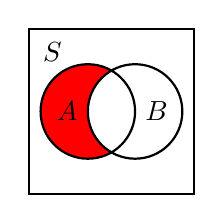
\begin{tikzpicture}[thick, scale=0.3]
  \draw (-3.5, -3.5) rectangle (3.5, 3.5);
\fill[red] (0,0 |- 60:2cm) arc [start angle=60, end angle = 300, radius = 2cm]
                           arc [start angle=240, end angle = 120, radius = 2cm];
  \draw (-1,0) circle [radius=2cm]
               (1,0) circle [radius=2cm];
  \draw (-1,0) node[left] {$A$};
  \draw (1,0) node[right] {$B$};
  \draw (-2.5,2.5) node {$S$};
\end{tikzpicture}
  \end{minipage}
    \begin{Example}
        $\{1,2\} \setminus \{2,3\} = \{1\}$
    \end{Example}
}

{\flushleft
\begin{minipage}{0.70\linewidth}
  \begin{Def}
    在许多实际问题中,常以某个集合$S$为出发点,而所涉及的集合都是$S$的子集。这个包含所考虑的所有集合的集合$S$,称为该问题的全集。如果$A$为$S$的子集,则差集$S \setminus A$称为集合$A$对集合$S$的余集,记为$A^c$。
    \begin{equation*}
      A^c = \{x|x \in S \land x \notin A\}
    \end{equation*}
  \end{Def}
\end{minipage}
\begin{minipage}{0.29\linewidth}
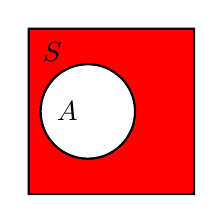
\begin{tikzpicture}[thick, scale=0.3]
  \filldraw[fill=red] (-3.5, -3.5) rectangle (3.5, 3.5)
               (-1, 0) circle [radius = 2cm];
  \draw (-1,0) node[left] {$A$};
  \draw (-2.5,2.5) node {$S$};
\end{tikzpicture}
\end{minipage}
}
    \begin{Example}
        $S = \{0,1\}, A =  \{0\},$ 则$A^c = \{1\}$
    \end{Example}

\begin{Thm}
设$S$为全集,$\emptyset$为空集,$A$,$B$,$C$为$S$的子集,则\\
1. $A \cup B = B \cup A$, $A \cap B = B \cap A$.\\
2. $(A \cup B) \cup C = A \cup (B \cup C)$,$(A \cap B) \cap C = A \cap (B \cap C)$.\\
%3. $A \cup A = A$,$A \cap A = A$.\\
%4. $(A \cup B) \cap A = A$,$(A \cap B) \cup A = A$.\\
4. $A \cup \emptyset = A$, $A \cap \emptyset = \emptyset$.\\
5. $A \cup S = S$, $A \cap S = A$.\\
6. $A \cap (B \cup C) = (A \cap B) \cup (A \cap C)$, $A \cup (B \cap C) = (A \cup B) \cap (A \cup C)$.\\
7. $A \cup A^c = S$, $A \cap A^c = \emptyset$.\\
8. $C\setminus (A \cup B) = (C \setminus A) \cap (C \setminus B)$, $C \setminus (A \cap B) = (C \setminus A) \cup (C \setminus B)$.\\ 
8'. $(A \cup B)^c = A^c \cap B^c$, $(A \cap B)^c = A^c \cup B^c$.\\
\end{Thm}
  以下只证明结论6的第一条,其他结论的证明留给读者自己完成。

  首先在草稿纸上做如下的分析。

  \begin{equation*}
    \begin{split}
      \forall x, &x \in A \cap (B \cup C) \\
      \Leftrightarrow& x \in A \land x \in (B \cup C)\\
      \Leftrightarrow& x \in A \land (x \in B \lor x \in C)\\
      \Leftrightarrow& (x \in A \land x \in B) \lor (x \in A \land x \in C)\\
      \Leftrightarrow& (x \in A \cap B) \lor (x \in A \cap C)\\
      \Leftrightarrow& x \in (A \cap B) \cup (A \cap C)
    \end{split}
  \end{equation*}
  然后将上面的分析转化为证明如下:  
\begin{proof}[证明]
  先证$A \cap (B \cup C) \subseteq (A \cap B) \cup (A \cap C)$。

  对任意的$x$,如果$x \in A \cap (B \cup C)$,则 $x \in A$并且$x \in (B \cup C)$,从而$x \in A$,并且$x \in B$或者$ x \in C$,
  因此,$x \in A$并且$x \in B$,或者$x \in A$并且$ x \in C$,即,$x \in A \cap B$ 或者$x \in A \cap C$,于是,$x \in (A \cap B) \cup (A \cap C)$。

  再证$(A \cap B) \cup (A \cap C) \subseteq A \cap (B \cup C)$。

    对任意的$x$,如果$x \in (A \cap B) \cup (A \cap C)$,则 $x \in A \cap B$ 或者$x \in A \cap C$,从而$x \in A$并且$x \in B$,或者$x \in A$并且$ x \in C$,
  因此,$x \in A$,并且$x \in B$或者$ x \in C$,即,$x \in A$并且$x \in (B \cup C)$,于是,$x \in A \cap (B \cup C)$。

\end{proof}
{\flushleft
\begin{minipage}{0.69\linewidth}
  \begin{Def}
    设$A,B$为任意的两个集合,$A\setminus B$与$B\setminus A$的并集称为$A$与$B$的对称差,记为$A \bigtriangleup B$。
    \begin{equation*}
      A\bigtriangleup B = (A \setminus B) \cup (B \setminus A)
    \end{equation*}
  \end{Def}
\end{minipage}
\begin{minipage}{0.29\linewidth}
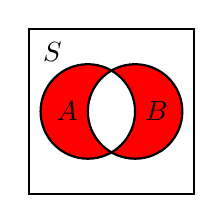
\begin{tikzpicture}[thick, scale=0.3]
  \draw (-3.5, -3.5) rectangle (3.5, 3.5);
\fill[red] (0,0 |- 60:2cm) arc [start angle=60, end angle = 300, radius = 2cm]
                           arc [start angle=240, end angle = 120, radius = 2cm];
\fill[red] (0,0 |- 60:2cm) arc [start angle=120, end angle = -120, radius = 2cm]
                           arc [start angle=-60, end angle = 60, radius = 2cm];
  \draw (-1,0) circle [radius=2cm]
               (1,0) circle [radius=2cm];
  \draw (-1,0) node[left] {$A$};
  \draw (1,0) node[right] {$B$};
  \draw (-2.5,2.5) node {$S$};
\end{tikzpicture}
  \end{minipage}}
    \begin{Example}
        $\{1,2\} \bigtriangleup \{2,3\} = \{1,3\}$
      \end{Example}

      \begin{Thm}
        设$S$为全集,$A\in 2^S$,$B\in 2^S$,则
        \begin{equation*}
          A \bigtriangleup B = (A \cap B^c)\cup (A^c \cap B)
        \end{equation*}
      \end{Thm}
  \begin{Thm}
设$S$为全集,$\emptyset$为空集,$A$,$B$,$C$为$S$的子集,则\\
1. $A \bigtriangleup B = B \bigtriangleup A$.\\
2. $(A \bigtriangleup B) \bigtriangleup C = A \bigtriangleup (B \bigtriangleup C)$.\\
3. $\emptyset \bigtriangleup A = A$.\\
4. $A \bigtriangleup A = \emptyset$.\\
5. $A \cap (B \bigtriangleup C) = (A \cap B) \bigtriangleup (A \cap C)$.\\ 
  \end{Thm}

\begin{proof}[证明]以下证明结论2,其他结论留给读者思考。
  
  因为
  \begin{equation}
  x \in A \bigtriangleup B \Leftrightarrow
  (x \in A \land x \notin B) \lor (x \notin A \land x
  \in B),    
  \end{equation}

  所以
  \begin{equation}
    \begin{split}
      x \notin A \bigtriangleup B &\Leftrightarrow
  (x \notin A \lor x \in B) \land (x \in A \lor x
  \notin B)\\
  &\Leftrightarrow (x \notin A \land x \notin B) \lor (x \in A \land x \in B )
    \end{split}
  \end{equation}

  于是
  \begin{equation}\label{xor1}
    \begin{split}
      &x \in (A \bigtriangleup B) \bigtriangleup C\\
      &\Leftrightarrow (x \in A \bigtriangleup B \land x \notin C) \lor (x \notin A \bigtriangleup B \land x \in C)\\
      &\Leftrightarrow (((x \in A \land x \notin B) \lor (x \notin A \land x \in B)) \land x \notin C)\\
      &\lor (((x \notin A \land x \notin B) \lor (x \in A \land x \in B )) \land x \in C)\\
      &\Leftrightarrow (x \in A \land x \notin B \land x \notin C) \lor (x \notin A \land x \in B \land x \notin C)\\
      &\lor (x \notin A \land x \notin B \land x \in C) \lor (x \in A \land x \in B \land x \in C)
    \end{split}
  \end{equation}

  \begin{equation}\label{xor2}
    \begin{split}
      &x \in A \bigtriangleup (B \bigtriangleup C)\\
      &\Leftrightarrow x \in (B \bigtriangleup C) \bigtriangleup A\\
      &\Leftrightarrow (x \in A \land x \notin B \land x \notin C) \lor (x \notin A \land x \in B \land x \notin C)\\
      &\lor (x \notin A \land x \notin B \land x \in C) \lor (x \in A \land x \in B \land x \in C)
    \end{split}
  \end{equation}
  其中\eqref{xor2}式的第二行由对称差运算的交换律得到,\eqref{xor2}式的第三行由与
   \eqref{xor1}式的对称性得到。

  由\eqref{xor1}式和\eqref{xor2}式可得
  $(A\bigtriangleup B)\bigtriangleup C = A\bigtriangleup (B\bigtriangleup C)$。
\end{proof}

  \begin{Def}  
    以集合为元素的集合称为集族。如果$I$为任意一个集合,对$I$中每个元素$\alpha$都有一个唯一的集合与之对应,这个集合记为$A_{\alpha}$,那么所有这些$A_{\alpha}$形成的集族可以用$\{A_{\alpha}\}_{\alpha \in I}$表示,其中$I$称为标号集。
  \end{Def}
  \begin{Def}
    集族$\{A_{\alpha}\}_{\alpha \in I}$中所有集合的并集$\bigcup_{\alpha \in I}A_{\alpha}$定义为
\[ \bigcup_{\alpha \in I}A_{\alpha} = \{x|\exists \alpha \in I \text{使得} x \in A_{\alpha}\}\]
    集族$\{A_{\alpha}\}_{\alpha \in I}$中所有集合的交集$\bigcap_{\alpha \in I}A_{\alpha}$定义为
\[ \bigcap_{\alpha \in I}A_{\alpha} = \{x|\forall \alpha \in I, x \in A_{\alpha}\}\]
  \end{Def}

  \begin{Example}
    设$I=\{x \in \mathbb{R} | 0 < x \leq 1\}$,$\forall x \in \mathbb{R}, A_x=\{y\in \mathbb{R}|0 < y < x\}$,
    则
    \begin{equation*}
      \bigcup_{x\in I}A_x=\{x \in \mathbb{R} | 0 < x \leq 1\},
      \bigcap_{x\in I}A_x=\phi      
    \end{equation*}
  \end{Example}

  \begin{Thm}
设$A$为任意集合, $\{B_{\alpha}\}_{\alpha \in I}$为任意一个集族,则
\begin{enumerate}
\item $A \cap (\bigcup_{\alpha \in I}B_{\alpha}) = \bigcup_{\alpha \in I}(A \cap B_{\alpha})$
\item $A \cup (\bigcap_{\alpha \in I}B_{\alpha}) = \bigcap_{\alpha \in I}(A \cup B_{\alpha})$
\item $(\bigcup_{\alpha \in I}A_{\alpha})^c=\bigcap_{\alpha\in I}A_{\alpha}^c$
\item $(\bigcap_{\alpha \in I}A_{\alpha})^c=\bigcup_{\alpha\in I}A_{\alpha}^c$
\end{enumerate}
\end{Thm}
  \begin{Def}
    两个对象按照一定的顺序排列构成的整体称为一个有序对。如果第一个对象为$a$ ,第二个对象为$b$ ,则该有序对记为$(a,b)$。$(a,b)=(c,d)$当且仅当$a=c$并且$b=d$。
  \end{Def}
  \begin{Def}
    设$A$与$B$为任意两个集合,则称集合 $\{(a,b)|a\in A \land b \in B\}$为$A$与$B$的笛卡尔乘积,记为$A \times B$。
即
\begin{equation*}
  A \times B = \{(a,b)|a \in A \land b \in B\}
\end{equation*}
  \end{Def}
  \begin{Example}
    如果$X=\{1,2\}$,$Y=\{3,4,5\}$,那么$X \times Y = ?$, $Y \times X = ?$
    \begin{equation*}
      \begin{split}
       X \times Y &= \{ (1,3), (1,4), (1,5), (2,3), (2,4), (2, 5) \}\\
       Y \times X &= \{(3,1), (3,2), (4,1), (4,2), (5,1), (5,2)\}
      \end{split}
    \end{equation*}
  \end{Example}

  \begin{Def}
    $n$个对象按照一定的顺序排列构成的整体称为一个$n$元组。如果第一个对象为$a_1$,第二个对象为$a_2$,$\ldots$,第$n$个对象为$a_n$,则该$n$元组记为$(a_1,a_2, \ldots, a_n)$。

 $(a_1,a_2, \ldots, a_n)=(b_1,b_2, \ldots, b_n)$当且仅当$a_1=b_1$,$a_2=b_2$,$\ldots$,$a_n=b_n$。
  \end{Def}
  \begin{Def}
    设$A_1$, $A_2$,$\ldots$,$A_n$为任意$n$个集合,则称集合 \[\{(a_1,a_2, \ldots, a_n)|a_i\in A_i, i = 1,2,\ldots, n\}\] 为$A_1, A_2, \ldots, A_n$ 的笛卡尔乘积,记为$A_1 \times A_2 \times \cdots \times A_n$, 简记为$\prod_{i=1}^nA_i$。即
\begin{equation*}
  A_1 \times A_2 \times \cdots \times A_n = \prod_{i=1}^nA_i = \{(a_1,a_2, \ldots, a_n)|a_i \in A_i, i = 1, 2, \cdots, n\}
\end{equation*}

当$A_1=A_2=\cdots=A_n=A$时,$A_1 \times A_2\times \cdots \times A_n$简记为$A^n$,例如$A^2=A\times A$,$A^3=A\times A\times A$。
我们以前熟知的二维空间$R^2$即为$R\times R$,三维空间$R^3$即为$R\times R\times R$。

  \end{Def}
  \begin{Example}
    如果$X=\{a_1,b_1\}$,$Y=\{a_2,b_2\}$,$Z=\{a_3,b_3\}$ 那么 $X \times Y \times Z = ?$
    \begin{equation*}
      \begin{split}
       X \times Y \times Z =& \{ (a_1,a_2, a_3), (a_1,a_2, b_3), (a_1, b_2, a_3), (a_1,b_2, b_3), \\
&(b_1, a_2, a_3), (b_1, a_2, b_3), (b_1, b_2, a_3), (b_1, b_2, b_3) \}\\
      \end{split}
    \end{equation*}
  \end{Example}

  \begin{Def}
    设$X$和$Y$为两个非空集合。一个从$X$到$Y$的映射$f$为一个法则,根据$f$,对$X$中的每个元素$x$都有$Y$中唯一确定的元素$y$与之对应。
    从$X$到$Y$的映射$f$常记为$f:X\to Y$。
  \end{Def}
    \begin{Def}
    设$f:X\to Y$,如果$\forall x_1, x_2 \in X$, 只要$x_1 \neq x_2$,  就 有 $f(x_1) \neq f(x_2)$,   则称 $f$为从$X$到$Y$的单射。
  \end{Def}
  \begin{Def}
    设$f:X\to Y$, 如果$\forall y \in Y$, $\exists x \in X$使得 $f(x) = y$, 则称$f$为从$X$到$Y$的满射。
  \end{Def}
  \begin{Def}
    设$f:X\to Y$,如果$f$既是单射又是满射,则称$f$为从$X$到$Y$的双射,或者称$f$为从$X$到$Y$的一一对应。
  \end{Def}

  \begin{Def}
设$A$为一个集合,如果$A=\Phi$,其基数定义为$0$;如果$A \neq \Phi$且存在一个自然数$n$使得$A$与集合$\{1,2,\ldots, n\}$之间存在一个一一对应,则定义$A$的基数为$n$。$A$的基数记为$|A|$。如果$|A|$为0或某个自然数$n$,则称
$A$为有穷集;如果A不是有穷集,则称$A$为无穷集。   
  \end{Def}
  \begin{Thm}
    设$A,B$为两个不相交的有穷集,则$|A \cup B| = |A| + |B|$。
  \end{Thm}
  \begin{Thm}
    设$A_1,A_2, \ldots, A_n$为$n$个两两不相交的有穷集,则\[|\bigcup_{i=1}^{n}A_i|=\sum_{i=1}^{n}|A_i|.\]
  \end{Thm}
  \begin{Thm}
    设$A,B$为有穷集,则$|A \times B| = |A| \cdot |B|$。
  \end{Thm}
  \begin{Thm}
    设$A_1,A_2, \ldots, A_n$为$n$个有穷集,则\[|A_1 \times A_2 \times \cdots \times A_n|=|A_1|\cdot |A_2| \cdot \cdots \cdot |A_n|.\]
  \end{Thm}
\begin{Thm}
  设$S$为有穷集,$A \subseteq S$, 则$|A^c| = |S| - |A|$。
\end{Thm}
\begin{Thm}
  设$A,B$为有穷集,则
$|A \cup B| = |A| + |B| - |A \cap B|$。
\end{Thm}

\begin{Thm}
  设$A_1, A_2, \ldots, A_n$为$n$个有穷集,则
  \begin{equation*}
\begin{split}
    &|\bigcup_{i=1}^nA_i|\\
=&\sum_{i=1}^n|A_i| - \sum_{1\leq i < j \leq n}|A_i \cap A_j| + \sum_{1 \leq  i < j < k \leq n}|A_i \cap A_j \cap A_k|\\
-&\ldots\\
+&(-1)^{n+1}|A_1 \cap A_2 \cap \cdots \cap A_n| 
  \end{split}
\end{equation*}
\end{Thm}
\begin{proof}[证明]
用数学归纳法证明,施归纳于$n$:

当$n=1$时,结论显然成立。

假设定理的结论对$n \geq 1$个有穷集合成立,往证对$n+1$个有穷集合定理的结论也成立。实际上,

  \begin{equation}\label{eq1}
    \begin{split}
      &|\bigcup_{i=1}^{n+1}A_i|\\
      =&|(\bigcup_{i=1}^nA_i) \cup A_{n+1}|\\
      =&|\bigcup_{i=1}^nA_i| + |A_{n+1}| - |(\bigcup_{i=1}^nA_i) \cap A_{n+1}|\\
      =&|\bigcup_{i=1}^nA_i| + |A_{n+1}| - |(A_1 \cap A_{n+1}) \cup (A_2 \cap A_{n+1}) \cup \cdots \cup (A_n \cap A_{n+1})|
    \end{split}
  \end{equation}

    由归纳假设
  \begin{equation}\label{eq2}
\begin{split}
    &|\bigcup_{i=1}^nA_i|\\
=&\sum_{i=1}^n|A_i| - \sum_{1\leq i < j \leq n}|A_i \cap A_j| + \sum_{1 \leq  i < j < k \leq n}|A_i \cap A_j \cap A_k|\\
-&\ldots\\
+&(-1)^{n+1}|A_1 \cap A_2 \cap \cdots \cap A_n| 
  \end{split}
\end{equation}

  \begin{equation}\label{eq3}
    \begin{split}
      &|(A_1 \cap A_{n+1}) \cup (A_2 \cap A_{n+1}) \cup \cdots \cup (A_n \cap A_{n+1})|\\
      =&\sum_{i=1}^n|A_i \cap A_{n+1}| - \sum_{1\leq i < j \leq n}|(A_i \cap A_{n+1}) \cap (A_j \cap A_{n+1}) |\\
      &+ \sum_{1 \leq  i < j < k \leq n}|(A_i \cap A_{n+1}) \cap (A_j \cap A_{n+1}) \cap (A_k \cap A_{n+1})|\\
&-\ldots\\
&+(-1)^{n+1}|(A_1 \cap A_{n+1}) \cap (A_2 \cap A_{n+1}) \cap \cdots \cap (A_n \cap A_{n+1})| \\
      =&\sum_{i=1}^n|A_i \cap A_{n+1}| - \sum_{1\leq i < j \leq n}|(A_i  \cap A_j \cap A_{n+1}) |\\
      &+ \sum_{1 \leq  i < j < k \leq n}|A_i  \cap A_j  \cap A_k \cap A_{n+1}|\\
&-\ldots\\
&+(-1)^{n+1}|A_1  \cap A_2  \cap \cdots \cap A_n \cap A_{n+1}| \\
    \end{split}
  \end{equation}
    将\eqref{eq2}和\eqref{eq3}代入\eqref{eq1}得
  \begin{equation*}
    \begin{split}
    &|\bigcup_{i=1}^{n+1}A_i|\\
=&\sum_{i=1}^{n+1}|A_i| - \sum_{1\leq i < j \leq {n+1}}|A_i \cap A_j| + \sum_{1 \leq  i < j < k \leq {n+1}}|A_i \cap A_j \cap A_k|\\
-&\ldots\\
+&(-1)^{n+1+1}|A_1 \cap A_2 \cap \cdots \cap A_{n+1}|
\end{split}
\end{equation*}


\end{proof}
\begin{Example}
  在1000名大学毕业生的调查中,每个人至少掌握了一门外语,其中804人掌握了英语,205人掌握了日语,190人掌握了 俄语,125人既掌握了英语又掌握了日语,57人既掌握了日语又掌握了俄语,85人既掌握了英语又掌握了俄语。试求在这1000名大学生中,英语、日语、俄语全掌握的有多少人?
\end{Example}

\begin{proof}[解]
  设$A,B,C$分别为掌握了英语、日语、俄语的大学生的集合,则
  \begin{equation*}
    \begin{split}
      &|A \cup B \cup C|\\
      = &|A| + |B| + |C|\\
      - & |A \cap B| - |A \cap C| - |B \cap C| + |A \cap B \cap C|\\
    \end{split}
  \end{equation*}
  即
  \begin{equation*}
    1000 = 804 + 205 + 190 - 125 - 85 - 57 +  |A \cap B \cap C|
  \end{equation*}
  解得英语、日语、俄语全掌握的人数$|A \cap B \cap C|=68$。
\end{proof}
  \begin{Exercise}
    设集合$A=\{1,2,3\}$,$B=\{2,3,4\}$,则$A\cup B=\underline{\quad\quad\quad}$,$A\cap B=\underline{\quad\quad\quad}$,$A\setminus B=\underline{\quad\quad\quad}$,$A\bigtriangleup B=\underline{\quad\quad\quad}$,$A\times B=\underline{\quad\quad\quad}$。
  \end{Exercise}
  \begin{Exercise}
    下列命题中哪个是假的?

    A. 对每个集合$A$,$\phi \in 2^A$。

    B. 对每个集合$A$,$\phi \subseteq 2^A$。

    C. 对每个集合$A$,$A \in 2^A$。

    D. 对每个集合$A$,$A \subseteq 2^A$。
  \end{Exercise}
    \begin{Exercise}
   设集合$S=\{\phi, \{\phi\}\}$,则$2^S=\underline{\quad\quad\quad}$。
  \end{Exercise}
  \begin{Exercise}
   设$A$,$B$,$C$为集合,证明:$(A\cup B) \setminus C = (A\setminus C) \cup
   (B\setminus C)$。
 \end{Exercise}
    \begin{Exercise}
      下列等式是否成立:$(A\cup B) \setminus C = A \cup (B\setminus C)$?
    \end{Exercise}

  \begin{Exercise}
下列命题中哪个是真的?

A. 对任何集合$A$,$B$,$2^{A\cup B} = 2^A \cup 2^B$。

B. 对任何集合$A$,$B$,$2^{A\cap B} = 2^A \cap 2^B$。

C. 对任何集合$A$,$B$,$2^{A\setminus B} = 2^A \setminus 2^B$。

D. 对任何集合$A$,$B$,$2^{A\bigtriangleup B} = 2^A \bigtriangleup 2^B$。
  \end{Exercise}
  \begin{Exercise}
    设$A$,$B$,$C$为集合,并且$A\cup B = A \cup C$,则下列哪个断言成立?

    A. $B = C$

    B. $A \cap B = A \cap C$

    C. $A \cap B^c = A \cap C^c$

    D. $A^c \cap B = A^c \cap C$
  \end{Exercise}
  \begin{Exercise}
    设$A$,$B$,$C$,$D$为任意四个集合,证明

    $(A \cap B) \times (C \cap D) =
    (A\times C) \cap (B \times D)$
  \end{Exercise}
  \begin{Exercise}
   设$A$,$B$,$C$为集合,化简

$(A \cap B \cap C)\cup (A^c \cap B \cap C) \cup (A \cap B^c \cap C) \cup (A \cap B \cap C^c) \cup (A^c \cap B^c \cap C) \cup (A \cap B^c \cap C^c) \cup (A^c \cap B \cap C^c)$
  \end{Exercise}
  \begin{Exercise}
   证明

1) $A\bigtriangleup B = (A\cup B) \cap (A^c \cup B^c)$

2) $(A \bigtriangleup B)^c = (A \cap B) \cup (A^c \cap B^c)$

3) $(A \bigtriangleup B)^c = (A^c \cup B) \cap (A \cup B^c)$
\end{Exercise}
\begin{Exercise}
  设$A,B,C$都是集合,若$A\cup B = A\cup C$且$A\cap B = A\cap C$,试证$B=C$。
\end{Exercise}
% \clearpage
% newtheorem{Exercise1}{练习}[chapter]
%   \begin{Exercise1}
%     设集合$A=\{1,2,3\}$,$B=\{2,3,4\}$,则$A\cup B=\underline{\{1,2,3,4\}}$,$A\cap B=\underline{\{2,3\}}$,$A\setminus B=\underline{\{1\}}$,$A\bigtriangleup B=\underline{\{1,4\}}$,$A\times B=\underline{\{(1,2),(1,3),(1,4),(2,2),(2,3),(2,4),(3,2),(3,3),(3,4)\}}$。
%   \end{Exercise1}
%   \begin{Exercise1}
%     下列命题中哪个是假的?(D)

%     A. 对每个集合$A$,$\phi \in 2^A$。

%     B. 对每个集合$A$,$\phi \subseteq 2^A$。

%     C. 对每个集合$A$,$A \in 2^A$。

%     D. 对每个集合$A$,$A \subseteq 2^A$。
%   \end{Exercise1}

%     \begin{Exercise1}
%    设集合$S=\{\phi, \{\phi\}\}$,则$2^S=\underline{\{\phi, \{\phi\}, \{\{\phi\}\}, \{\phi, \{\phi\}\}}$。
%   \end{Exercise1}

%   \begin{Exercise1}
%    设$A$,$B$,$C$为集合,证明:$(A\cup B) \setminus C = (A\setminus C) \cup
%    (B\setminus C)$。
%  \end{Exercise1}
%   \begin{proof}[证明]
%    先证$(A\cup B) \setminus C \subseteq (A\setminus C) \cup
%    (B\setminus C)$。

%    对任意的$x$,如果$x \in (A\cup B) \setminus C$,则$x \in (A\cup B)$并且$x
%    \notin C$,从而$x \in A$或者$x \in B$,并且$x \notin C$,即$x \in A$并
%    且$x \notin C$成立,或者$x \in B$并且$x \notin C$成立。于是,$x \in A
%    \setminus C$或者$x \in B \setminus C$,因此,$x \in (A\setminus C) \cup
%    (B\setminus C)$。

%    再证 $(A\setminus C) \cup
%    (B\setminus C) \subseteq (A\cup B) \setminus C$。

%    对任意的$x$,如果$x \in (A\setminus C) \cup
%    (B\setminus C)$,则$x \in A
%    \setminus C$或者$x \in B \setminus C$,从而$x \in A$并
%    且$x \notin C$成立,或者$x \in B$并且$x \notin C$成立,即$x \in A$或者$x \in
%    B$,并且$x \notin C$,于是$x \in (A\cup B)$并且$x
%    \notin C$, 因此$x \in (A\cup B) \setminus C$。
%  \end{proof}

%     \begin{Exercise1}
%       下列等式是否成立:$(A\cup B) \setminus C = A \cup (B\setminus C)$?
%     \end{Exercise1}

%     \begin{proof}[解]
%       该等式不成立。举反例如下:设$A = \{1\}, B = \{1\}, C=\{1\}$,则$(A
%       \cup B)\setminus C = \phi $,而$A \cup (B\setminus C) = \{1\}$, 
% 此时$(A\cup B) \setminus C \neq A \cup (B\setminus C)$。
%     \end{proof}

\chapter{}
%%% Local Variables:
%%% mode: latex
%%% TeX-master: "book_chapter1"
%%% End:
